\begin{filecontents*}[overwrite]{refs.bib}
@misc{Geitgey_face_recognition,
  author={A. Geitgey},
  title={Face Recognition},
  year={2022},
  url={{https://github.com/ageitgey/face\_recognition}},
  urldate = {2022-08-12}
}

@misc{corso,
  author={A.M. Rinaldi},
  title={Slide Corso},
  year={2022},
}

@misc{docker,
  author={docker},
  title={Docker},
  year={2022},
  url={{https://www.docker.com/}},
  urldate = {2022-08-12}
}

@article{albiol2008face,
  title={Face recognition using HOG--EBGM},
  author={Albiol, Alberto and Monzo, David and Martin, Antoine and Sastre, Jorge and Albiol, Antonio},
  journal={Pattern Recognition Letters},
  volume={29},
  number={10},
  pages={1537--1543},
  year={2008},
  publisher={Elsevier}
}

@inproceedings{viola2001rapid,
  title={Rapid object detection using a boosted cascade of simple features},
  author={Viola, Paul and Jones, Michael},
  booktitle={Proceedings of the 2001 IEEE computer society conference on computer vision and pattern recognition. CVPR 2001},
  volume={1},
  pages={I--I},
  year={2001},
  organization={Ieee}
}

@inproceedings{cocskun2017face,
  title={Face recognition based on convolutional neural network},
  author={Co{\c{s}}kun, Musab and U{\c{c}}ar, Ay{\c{s}}eg{\"u}l and Yildirim, {\"O}zal and Demir, Yakup},
  booktitle={2017 International Conference on Modern Electrical and Energy Systems (MEES)},
  pages={376--379},
  year={2017},
  organization={IEEE}
}

@misc{Capasso_sm_2022,
  author = {Capasso, Giuseppe},
  month = {8},
  title = {{sm}},
  url = {https://github.com/alarmfox/sm},
  version = {1.0.0},
  year = {2022}
}

@misc{compose,
  title = {{Docker Compose}},
  url = {https://docs.docker.com/compose/},
  urldate = {2022-08-12}
}

@article{cheng2001color,
  title={Color image segmentation: advances and prospects},
  author={Cheng, Heng-Da and Jiang, X\_ H\_ and Sun, Ying and Wang, Jingli},
  journal={Pattern recognition},
  volume={34},
  number={12},
  pages={2259--2281},
  year={2001},
  publisher={Elsevier}
}

@misc{dlib,
  title = {dlib},
  url = {http://dlib.net/},
  urldate = {2022-08-11}
}

@misc{wiki:gradient,
  title = "Image Gradient --- {W}ikipedia{,} The Free Encyclopedia",
  author = {{Image Gradient}},
  url = {https://en.wikipedia.org/wiki/Image\_gradient},
  urldate = {2022-08-12}
}

@misc{wiki:euclidean,
  title = "Euclidean Distance --- {W}ikipedia{,} The Free Encyclopedia",
  author = {{Euclidean Distance}},
  url = {https://en.wikipedia.org/wiki/Euclidean\_distance},
  urldate = {2022-08-16}
}

@misc{web:rest,
  title = "REST API",
  author = {{Redhat}},
  url = {https://www.redhat.com/it/topics/api/what-is-a-rest-api},
  urldate = {2022-08-12}
}

@misc{web:redis,
  title = "Redis",
  author = {{Redis}},
  url = {https://redis.io/},
  urldate = {2022-08-13}
}

@misc{web:opencv,
  title = "Opencv",
  author = {{Opencv}},
  url = {https://opencv.org/},
  urldate = {2022-08-13}
}
\end{filecontents*}

\documentclass{article}

\usepackage[utf8]{inputenc}
\usepackage[T1]{fontenc}
\usepackage{enumitem}
\usepackage{graphicx}
\usepackage[font=small,labelfont=bf]{caption}
\usepackage[italian]{babel}
\usepackage{amsmath}
\usepackage{url}
\usepackage[hidelinks]{hyperref}
\usepackage{apacite}
\usepackage[noabbrev]{cleveref}
\usepackage[margin=1in]{geometry}


\crefformat{subsection}{\S#2#1#3}
\crefformat{subsubsection}{\S#2#1#3}
\crefformat{figure}{#2Figura~#1#3}
\crefformat{footnote}{#2\footnotemark[#1]#3}

\begin{document}

\begin{titlepage}
    \begin{center}
        \vspace*{1cm}

        {\Huge\bfseries Progetto Sistemi Multimediali\par}

        \vspace{0.5cm}

        {\LARGE Face recognition over HTTP\par}

        \vfill

        {\Large Giuseppe Capasso\\
        N46003195\par}

        \vspace{0.8cm}
    \end{center}
\end{titlepage}

\tableofcontents
\listoffigures
\clearpage

\section{Introduzione}

Con la facilità di gestione delle informazioni dei moderni sistemi informativi e l'avvento della domotica, il tema del controllo degli accessi negli spazi è diventato sempre più presente nelle infrastrutture intelligenti e altamente automatizzate. In particolare, in campo \textit{enterprise}, si preferisce gestire le informazioni in maniera centralizzata ed essere indipendenti dal numero di accessi da monitorare. In quest'ottica il sistema proposto nel capitolo \ref{s:system} offre un punto unico da cui poter gestire utenti e accessi, facilmente integrabile in qualsiasi interfaccia grafica grazie all'astrazione fornita dalla rete.

Il sistema si occuperà di acquisire le immagini degli utenti grazie ad uno scanner posto agli ingressi da monitorare ed effettuerà il \textit{matching} dei volti riconosciuti con quelli autorizzati durante una fase di registrazione preliminare.
In particolare, lo scopo di questo progetto è quello di fornire una soluzione che sia:
\begin{itemize}
    \item di facile integrazione con sistemi di autenticazione di terze parti;
    \item indipendente dal numero e tipologia di dispositivi fisici;
    \item di facile installazione in locale;
\end{itemize}

Nel seguente elaborato, saranno affrontati i problemi relativi alla gestione centralizzata degli accessi focalizzandosi su:
\begin{itemize}
    \item invio e ricezione di immagini attraverso la rete;
    \item riconoscimento dei volti all'interno di un'immagine;
    \item memorizzazione dei meta-data dei volti all'interno di un database relazionale;
    \item confronto di due volti per confermare l'identità di una persona;
\end{itemize}

\section{Specifica delle metodologie}

\subsection{Segmentazione}
La segmentazione è il processo di divisione di un'immagine in regioni omogenee \cite[p.~1]{cheng2001color} ed è alla base del \textit{pattern recognition}. In generale, si tratta di applicare un predicato di omogeneità ad ogni pixel\footnote{Come mostrato di seguito, le tecniche di segmentazione vengono applicate a regioni di pixel.} per capire se appartiene ad una regione o meno. Formalmente, detto $F$ l'insieme dei pixel che costituisce l'immagine di partenza, la segmentazione divide $F$ in $n$ partizioni $S_i$ tale che:

\begin{equation}
    \bigcup\limits_{i=1}^{n} S_{i} =  F
\end{equation}

con $S_i \cap S_j = \emptyset$, per ogni $i \neq j$.

Le tecniche di segmentazione si basano sulla ricerca di discontinuità, linee, punti isolati e cambiamenti bruschi nella scala dei grigi \cite[p.~2]{cheng2001color}. In genere, gli approcci basilari nascono per trattare immagini monocromatiche, ma vengono combinati e adattati per essere utilizzati anche con le immagini a colori.

\subsubsection{Principali tecniche di segmentazione}
Di seguito viene effettuata una panoramica delle principali tecniche di segmentazione analizzando le differenze degli approcci con immagini a colori e monocromatiche.

\paragraph{Histogram thresholding}
Questa tecnica consiste nel calcolare l'istogramma di un'immagine e suddividere le regioni in base ai picchi che superano un certo valore di soglia (\textit{threshold}). L'utilizzo di questa tecnica per le immagini a colori si basa sulla sua trasposizione in campo multidimensionale. Inoltre, per le immagini a colori è molto importante scegliere lo spazio dei colori \cite[p.~3]{cheng2001color} e dipende dal tipo di immagine che si sta considerando.

\paragraph{Approcci region based} Questi approcci includono il \textit{region growing} e il \textit{region splitting}. Il primo si basa sulla scelta arbitraria di una regione e si procede ad espanderla fino a che il predicato non risulta falso, in tal caso ci si trova in un'altra regione. Il secondo, invece, considera come prima regione tutta l'immagine e se non è omogenea allora viene divisa in 4 parti e il processo ricomincia. Il primo approccio dipende fortemente dalla scelta della regione iniziale, mentre il secondo può portare a risultati troppo \textit{squadrati}. Entrambi gli approcci dipendono dalla scelta iniziale della regione, ma sono più robusti a disturbi poiché l'omogeneità di una regione è una proprietà calcolata statisticamente. Per le immagini a colori viene proposto un approccio misto tra \textit{region growing} e \textit{region splitting} unito al calcolo della distanza euclidea \cite{wiki:euclidean} tra le informazioni RGB per l'omogeneità di colore. Successivamente, per ogni area, vengono confrontati i pixel con quelli vicini per trovare eventuali disomogeneità. Quest'approccio per le immagini a colori è soggetto alla scelta delle soglie (che dipendono dal tipo di immagine) e non è applicabile alle immagini con ombre.

\paragraph{Edge detection} Questa tecnica consiste nel calcolare i livelli di discontinuità della scala di grigi e può essere applicata in due varianti: \textbf{sequenziale} (i risultati dei punti segnati dipendono da quelli precedentemente analizzati) o \textbf{parallela} (tutti i punti possono essere segnati in maniera indipendente da altri). Un cambiamento brusco in una scala di grigi implica che c'è un cambiamento di illuminazione nell'immagine.\\
Nelle immagini a colori, il cambiamento brusco deve avvenire in uno spazio tridimensionale per, ad esempio, riconoscere un oggetto. Al fine di riutilizzare quanto detto in precedenza, alcuni metodi riportano il problema nel caso monodimensionale o dando una definizione di distanza tra i colori o analizzando tre immagini separatamente (una per ogni colore) e combinando i risultati. Un approccio più sofisticato è quello di imporre delle condizioni sui valori dei tre colori in modo tale da analizzare l'immagine una sola volta.

\subsection{Riconoscimento facciale}
Le principali tecniche utilizzate per il riconoscimento facciale sono: Histogram of Oriented Gradients (HOG) e Convolutional Neural Network (CNN). In generale, il metodo HOG viene preferito al CNN quando ci sono risorse hardware limitate, ma risulta meno preciso in presenza di occlusioni, luci molto forti o cambiamenti di posa.\\
In questo elaborato, per contenere i costi di installazione e migliorare le prestazioni del sistema, la tecnica utilizzata è quella HOG. Infatti, l'uso di una CNN produce risultati più precisi, ma in tempi ragionevoli solo se può sfruttare l'accelerazione GPU/CUDA e rallenterebbe di molto il sistema nel caso di singola CPU \cite{Geitgey_face_recognition}.\\
Questa considerazione è un buon compromesso perché nel caso di un sistema di accesso ad una struttura luce e fotocamera possono essere progettati adeguatamente per garantire sempre la stessa qualità dell'immagine.

\subsubsection{Histogram Oriented Gradients}
Un descrittore HOG è una statistica locale degli orientamenti dei gradienti\footnote{Il gradiente di un insieme di pixel è la direzione del cambiamento dei colori \cite{wiki:gradient}.} di un'immagine intorno a un punto particolare \cite[p.~2]{albiol2008face}.

L'estrazione di \textit{feature} con il metodo HOG prevede la divisione dell'immagine in aree collegate e per ciascuno di esse viene calcolata un istogramma di orientamento (\cref{fig:hog}). Ogni area ha una grandezza in pixel predefinita e in base alla distanza media tra i due occhi, vengono calcolati i punti del volto applicando l'algoritmo in \cite[sez.~3.2]{albiol2008face} (\cref{fig:eye}).\\
La tecnica presente in \cite[sez.~3.2]{albiol2008face} presuppone la conoscenza della posizione degli occhi. Questo problema è risolto utilizzando il metodo in \cite[p.~5]{viola2001rapid}.

\begin{figure}[ht]
    \centering
    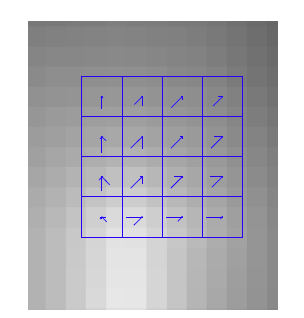
\includegraphics{images/hog.png}
    \caption{Direzionamento degli istogrammi in HOG}
    \label{fig:hog}
\end{figure}

\begin{figure}
    \centering
    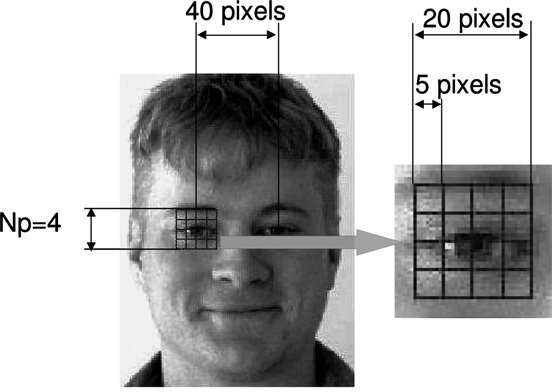
\includegraphics{images/albiol2008_3.jpg}
    \caption{HOG dell'occhio destro}
    \label{fig:eye}
\end{figure}

\subsection{Tecnologie utilizzate}
\subsubsection{Python}
Python è un linguaggio di programmazione interpretato \textit{general purpose} che fornisce una modalità semplice per effettuare \textit{binding} con moduli nativi. Questo lo rende adatto allo sviluppo di \textit{wrapper} di librerie di basso livello scritte in C/C++ quali \textit{opencv, dlib, numpy}. Inoltre, la sua componente di alto livello comporta una facilità di sviluppo per le applicazioni che utilizzano la rete.

\paragraph{Numpy}\label{p:numpy}
\textit{Numpy} è una libreria che offre le funzionalità matematiche avanzate. All'interno dell'applicazione, la libreria è utilizzata (congiuntamente ad \textit{opencv}) per decodificare le immagini in JPEG che arrivano dalla rete e per il calcolo della distanza vettoriale degli \textit{encoding} di due volti.
Infatti, le immagini trasmesse e ricevute attraverso la rete sono \textit{array} di \textit{byte} che, con Numpy, possono essere interpretati in \textit{uint8} (numeri a 8 bit senza segno, assume valori da 0 a 255) \cite{corso} con la funzione \textbf{frombuffer}. Inoltre, la funzione \textbf{argmin} sarà utilizzata per calcolare il minimo tra i riscontri ottenuti durante il riconoscimento facciale per ottenere il miglior risultato possibile.

\paragraph{Opencv}
\textit{Opencv} \cite{web:opencv} è una libreria open-source per la computer vision che offre gli strumenti per manipolare segnali multimediali. In questo progetto, sono utilizzate le sue funzioni di manipolazione delle immagini per:
\begin{itemize}
    \item codificare e decodificare le immagini che arrivano dalla rete in JPEG (funzioni \textbf{imencode} e \textbf{imdecode});
    \item preparare le immagini per il riconoscimento facciale, come richiesto dalla libreria \textit{face\_recognition};
    \item salvare le immagini relative agli accessi sul file-system (funzione \textbf{imwrite});
    \item evidenziare i volti degli utenti disegnando dei rettangoli sull'immagine di partenza;
\end{itemize}

Come accennato in \cref{p:numpy}, le immagini arrivano dalla rete come \textit{byte buffer} e con la funzione \textit{imdecode} di opencv possono essere decodificate in immagini a colori. Analogamente, per rispondere con un'immagine ad una richiesta di riconoscimento, viene utilizzata la funzione \textit{imencode}\footnote{Come spiegato in seguito, il sistema tratterà solo immagini JPEG}.

\paragraph{Face Recognition}\label{p:face_recognition}
Face recognition è una libreria basata su \textit{dlib} per il riconoscimento facciale. La libreria \textit{dlib} mette a disposizione algoritmi di \textit{machine learning} ed è scritta in C++ \cite{dlib}.\\
Questo modulo utilizza un modello che ha una precisione del 99.38\% \cite{Geitgey_face_recognition} e permette di utilizzare sia HOG che CNN. All'interno del prototipo sono utilizzate le seguenti funzioni:
\begin{itemize}
    \item \textbf{face\_locations}: data in ingresso un'immagine RGB\footnote{Opencv usa immagini in BGR, pertanto è necessaria una conversione.} ritorna una lista di coordinate che individuano i volti nell'immagine passata in ingresso;
    \item \textbf{face\_encodings}: dati in ingresso l'immagine iniziale e la lista di coordinate calcolata con \textit{face\_locations} ritorna una lista di \textit{encoding} a 128 dimensioni in cui ogni elemento rappresenta un volto nell'immagine;
    \item \textbf{compare\_faces}: dati gli \textit{encoding} dei volti già conosciuti, effettua un match con quelli da sconosciuti e ritorna una lista di valori booleani a seconda dell'esito del riscontro;
    \item \textbf{face\_distance}: ritorna la distanza tra l'\textit{encoding} del volto sconosciuto e quelli già conosciuti. Su queste distanze, sarà poi calcolato il minimo, come indicato in precedenza;
\end{itemize}

\paragraph{FastAPI}
FastAPI è un \textit{framework} per la realizzazione di servizi basati sul protocollo HTTP. In questo progetto, è utilizzato per esporre sulla rete le funzionalità del sistema di accessi. Inoltre, questo \textit{framework} produce una documentazione \textit{Swagger}\footnote{Questa documentazione è conforme allo standard OpenAPI 3.} per testare gli \textit{endpoint} interattivamente. Ad esempio, in \cref{fig:swagger_general}, sono mostrati gli \textit{endpoint} implementati per il prototipo.

\begin{figure}[ht]
    \centering
    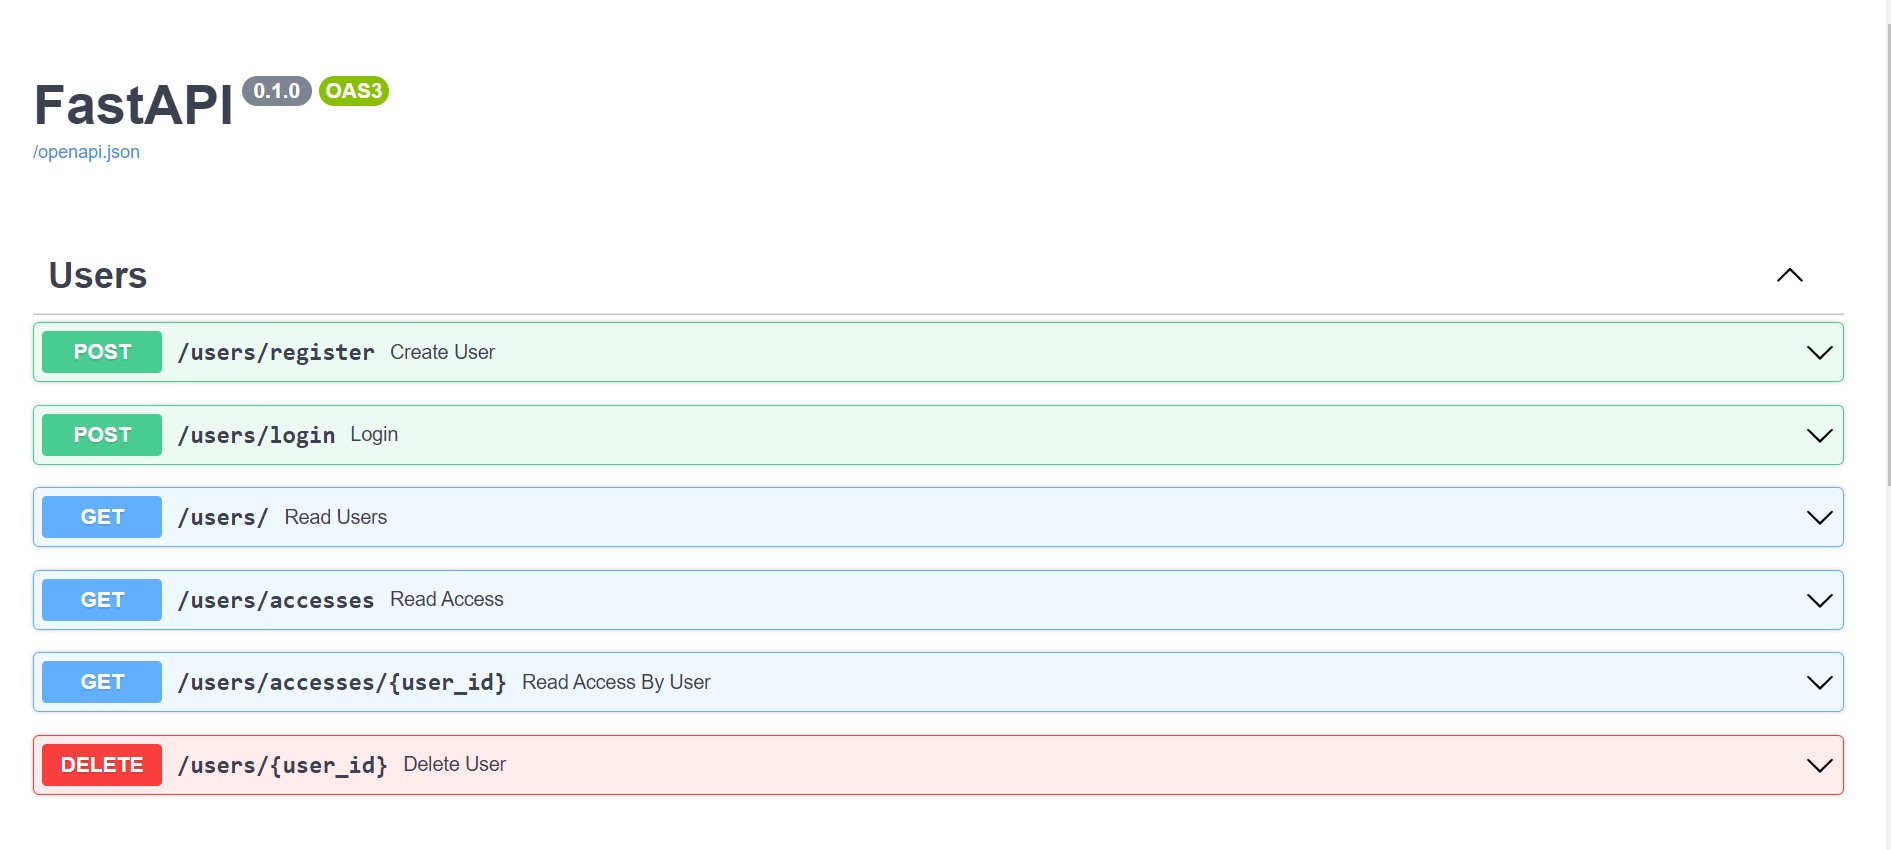
\includegraphics[width=\textwidth]{images/swagger_generale.png}
    \caption{Endpoint implementati mostrati nella Swagger UI}
    \label{fig:swagger_general}
\end{figure}

\subsubsection{PostgreSQL}
PostgreSQL è un database relazionale open-source utilizzato per conservare i dati degli utenti e quelli degli accessi. Il supporto per il tipo \textbf{byte array} è particolarmente utile per memorizzare gli \textit{encoding} (\textit{128-dimensional array}) estratti dai volti con la libreria \textit{face\_recognition} (\cref{p:face_recognition}).\footnote{Il processo di serializzazione e deserializzazione avviene con la libreria Python \textit{pickle}.}

\subsubsection{Redis}
Redis è una cache chiave-valore ad alte performance con supporto per il clustering\footnote{Più istanze possono essere usate per distribuire il carico su più macchine} \cite{web:redis}. In questo progetto, la cache viene utilizzata per velocizzare le \textit{query} dell'applicazione quando bisogna caricare gli \textit{encoding} dei volti dal database.

\subsubsection{Docker}
Docker \cite{docker} è una tecnologia che consente di installare le applicazioni in \textit{container}. Un container può essere visto come una macchina virtuale leggera che opera in un ambiente \textit{Linux} completamente isolato, ma condivide con l'host il kernel e le risorse hardware. Questo rende i Docker container leggeri e facilmente gestibili (creazione, eliminazione, allocazione risorse etc.) viste come applicazioni nello spazio utente. \\Un container è un'istanza di un'immagine Docker in esecuzione. La creazione di un'immagine è un processo che garantisce la riproducibilità dei progetti in ambienti isolati. Infatti, il prototipo proposto nel capitolo successivo può essere installato in un'immagine Docker (in cui sono eseguiti tutti i passi per installare le dipendenze necessarie) e, pertanto, eseguito su qualsiasi macchina su cui è installato Docker. Inoltre, Docker offre anche un sistema di \textit{networking} virtuale per far comunicare in maniera semplice i container.\\
Per il prototipo, è stato utilizzato \textit{docker-compose}\footnote{Docker Compose è uno script che automatizza l'inizializzazione di più container utilizzando un file \textit{yaml}.} \cite{compose}. In questo modo, viene automatizzata l'installazione del prototipo\footnote{Come spiegato in seguito, il prototipo consiste in un'applicazione Python, un database PostgreSQL e una cache Redis.}.

\section{Sistema}\label{s:system}
L'architettura logica del sistema è mostrata in \cref{fig:logical_arch}.

\begin{figure}[h]
  \centering
  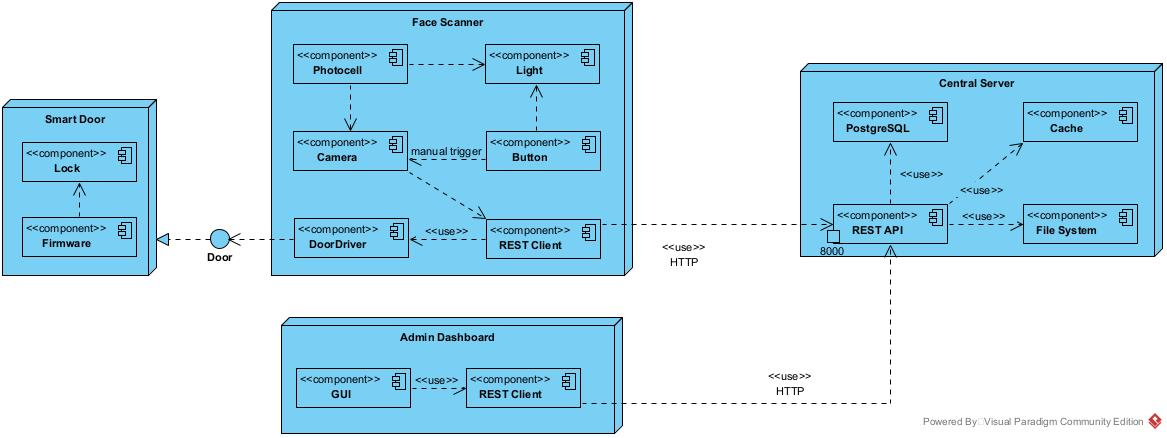
\includegraphics[width=\textwidth]{images/system.jpg}
  \caption{Architettura logica del sistema}
  \label{fig:logical_arch}
\end{figure}

Il sistema è composto dai seguenti componenti:
\begin{enumerate}
    \item \textbf{Central Server}: si occupa di memorizzare i visi e i dati degli utenti e offre una REST API \cite{web:rest} ai dispositivi fisici per effettuare il riconoscimento di un volto scansionato e agli amministratori per gestire accessi e utenti. \`E dotato sia di un database relazionale per lo storage permanente dei dati che di una cache per velocizzare i tempi di lettura e alleggerire il carico sul database. In questo componente è concentrata tutta la logica di \textit{backend};
    \item  \textbf{Admin Dashboard}: applicazione dotata di GUI utilizzata dagli amministratori di sistema per gestire gli utenti e visionare gli accessi. In questo componente è concentrata la logica \textit{frontend} per l'amministratore di sistema;
    \item \textbf{Face Scanner}: racchiude tutti i dispositivi fisici che servono a catturare un'immagine quando una persona desidera entrare nella struttura. Inoltre, in questo componente è presente un modulo software che consente di interagire, attraverso il protocollo HTTP, con il \textit{Central Server}. Idealmente, è formata dai seguenti dispositivi:
    \begin{itemize}
        \item \textit{Photocell}: dispositivo che rileva la presenza di una persona ed aziona la fotocamera per catturare l'immagine;
        \item \textit{Camera}: dispositivo posizionato per catturare, in primo piano, il volto della persona che desidera entrare;
        \item \textit{Light}: sorgente di illuminazione che viene attivata dalla fotocella per consentire l'accesso anche in condizione di scarsa luminosità;
        \item \textit{Button}: pulsante per azionare manualmente la scansione del volto, nel caso in cui ci fossero problemi con la fotocella;
    \end{itemize}
    \item \textbf{Smart door}: porta la cui serratura può essere sbloccata con un segnale elettrico. In generale, la porta è in grado di ricevere impulsi di apertura e chiusura e replicarli fisicamente sulla serratura.
\end{enumerate}

In generale, come si vede in \cref{fig:logical_arch}, la modalità fisica dello sblocco della serratura è indipendente dal sistema di autenticazione. Questo permette di utilizzare porte già presenti, ad esempio, installando una scheda elettronica con gli appositi collegamenti seriali.

Il focus di questo elaborato verte sul componente \textit{Central Server} (\cref{fig:central_server})\footnote{Il package DB contiene le classi che rappresentano la struttura del database spiegata in \cref{fig:er} omesse per semplicità.} e, in particolare:
\begin{itemize}
    \item sulla risoluzione del problema della ricezione e trasmissione delle immagini sulla rete;
    \item sull'individuazione e riconoscimento dei volti;
    \item sulla memorizzazione di meta-data sui volti in un database relazionale;
\end{itemize}

\begin{figure}[h]
\centering
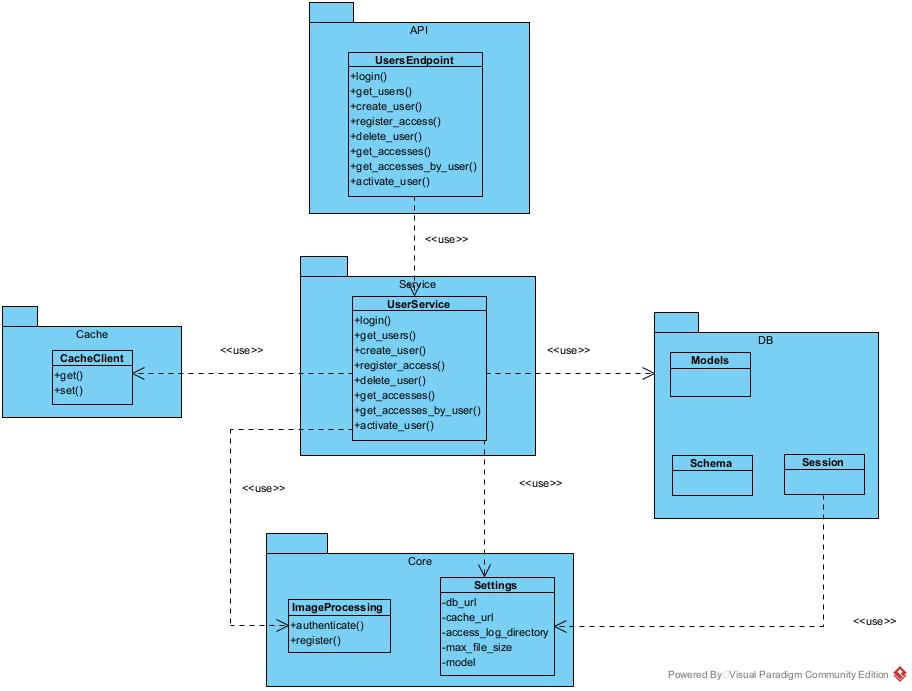
\includegraphics[width=\textwidth]{images/cs.jpg}
\caption{Struttura interna (semplificata) del \textit{Central Server}}
\label{fig:central_server}
\end{figure}

Pertanto, saranno trascurati tutti gli aspetti sulla sicurezza degli endpoint HTTP che non sono protetti da nessuna forma di autenticazione.
In particolare, affinché la soluzione sia completa, sarà necessario implementare un sistema di autenticazione che assicuri che solo gli utenti con i giusti privilegi possono accedere al registro degli accessi e alla gestione degli utenti (mediante l'uso di \textit{cookies}); mentre sarà necessario implementare un'autenticazione \textit{machine-to-machine} per far comunicare in maniera sicura server centrale e face scanner. Infine, sarà necessario esporre il servizio con il protocollo HTTPS per rendere cifrate le connessioni.

\subsection{Prototipo}
Il \textit{Central Server} consiste in un'applicazione \textit{Python} gestita con \textit{Miniconda}, un database PostgreSQL (lo schema di riferimento è mostrato in \cref{fig:er}) e una cache Redis.

Per le informazioni testuali (utili per costruire un'interfaccia grafica) il server utilizza la codifica JSON.

\begin{figure}[ht]
    \centering
    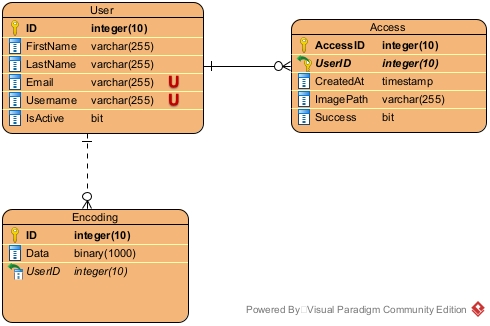
\includegraphics[width=\textwidth]{images/er.jpg}
    \caption{Modello ER del database relazionale utilizzato}
    \label{fig:er}
\end{figure}

Gli endpoint utilizzano le funzioni nel file \textit{utils.py} per non consentire all'utente di caricare immagini troppo grandi per evitare di degradare le performance del sistema.

Il prototipo realizzato implementa le seguenti funzionalità:
\begin{itemize}
    \item \textbf{login}: il server riceve un'immagine in JPEG e individua i volti all'interno di questa. Il sistema consente l'accesso se almeno uno dei volti individuato corrisponde con uno di quelli salvati;
    \item \textbf{gestione utenti}: il server permette di creare, leggere\cref{pagination}, cancellare e riattivare utenti\footnote{Nel prototipo un utente può essere sia disattivato che completamente eliminato. Un utente non attivo non può accedere alla struttura, ma resta memorizzato il suo storico accessi e può essere riattivato successivamente.} (\cref{fig:creazione_utente});
    \item \textbf{gestione accessi}: il server permette di ricevere la lista degli accessi (\cref{fig:get_accesses}) sia totale che per uno specifico utente\footnote{\label{pagination}Gli \textit{endpoint} che leggono le informazioni dal database utilizzano la paginazione: attraverso i parametri \textit{skip} e \textit{limit} consentono di limitare la quantità di record caricati dal database.};
\end{itemize}

Per rendere l'applicazione più realistica, sarà possibile selezionare gli accessi specificando un eventuale intervallo temporale di interesse (con granularità giornaliera).

\begin{figure}[ht]
\centering
    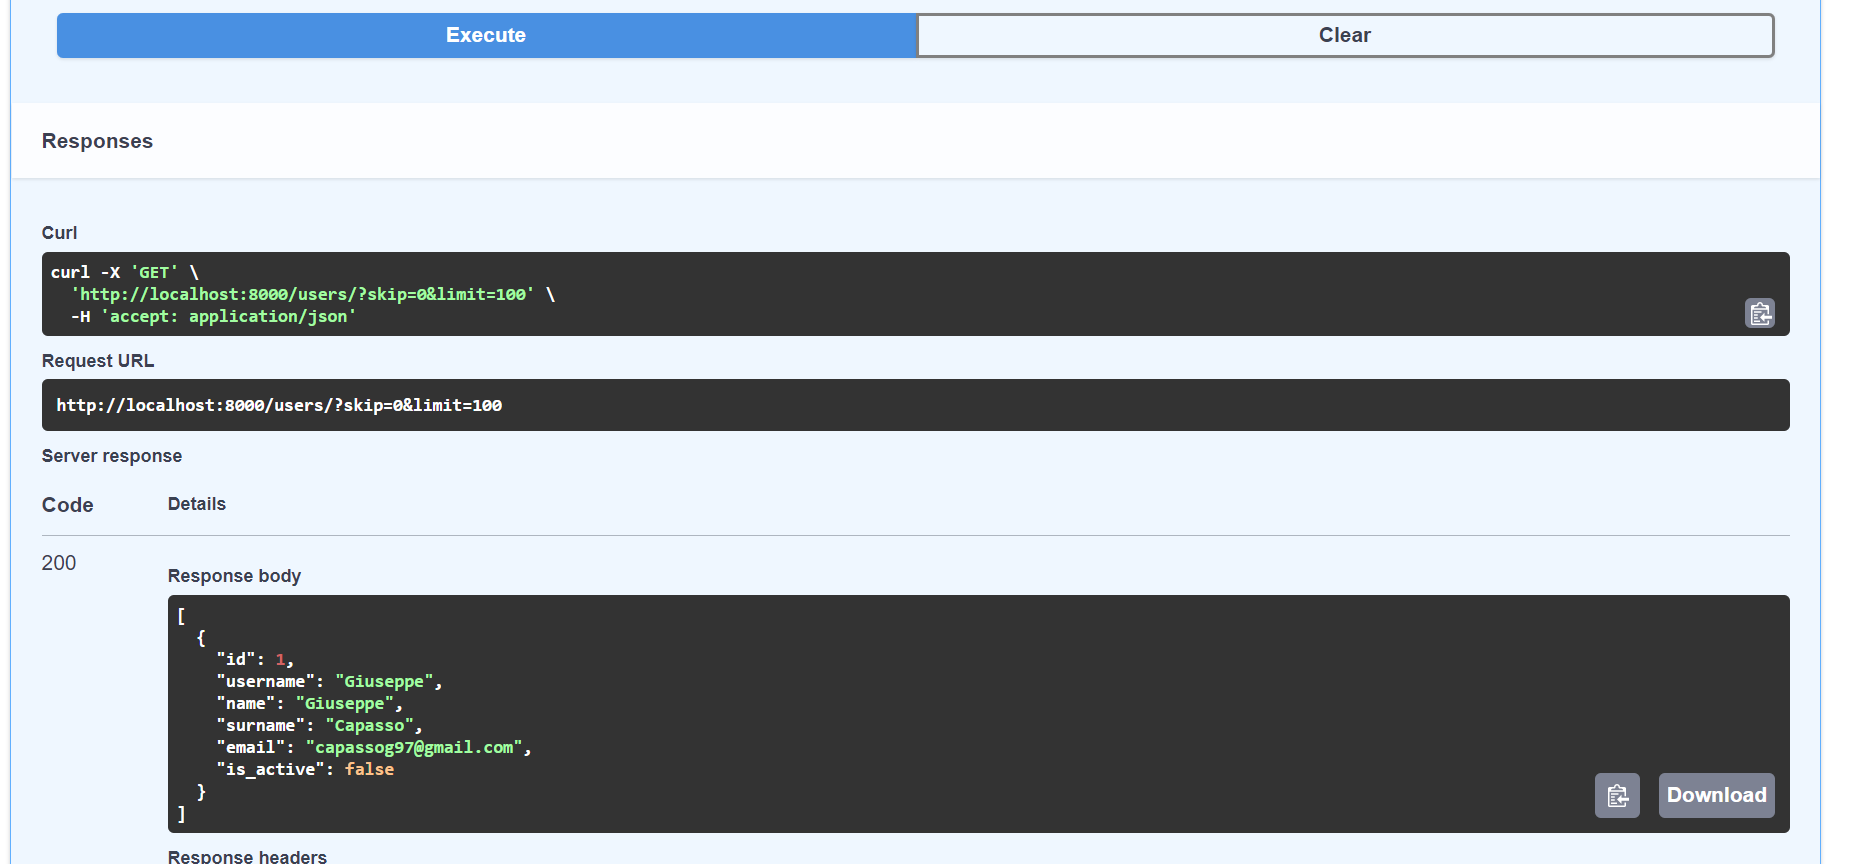
\includegraphics[width=\textwidth]{images/get_users.png}
    \caption{Lettura degli utenti dal database}
    \label{fig:get_users}
\end{figure}

\begin{figure}[ht]
\centering
    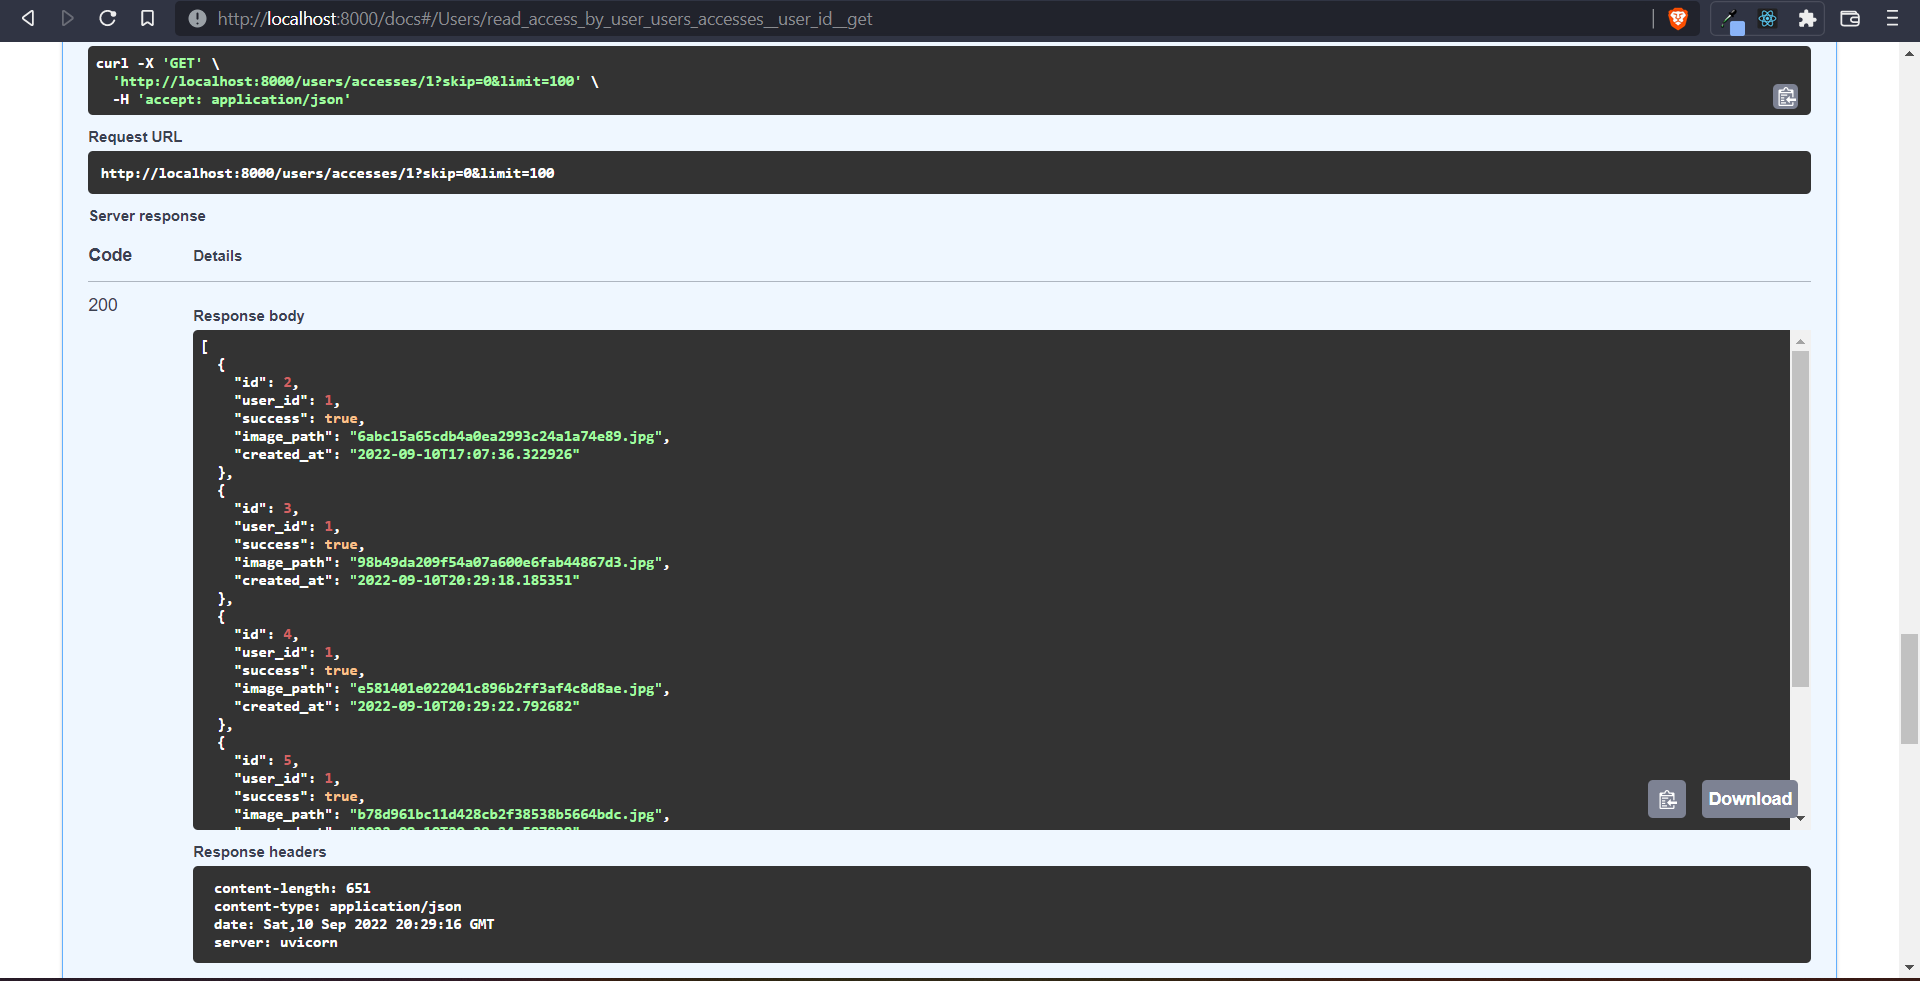
\includegraphics[width=\textwidth]{images/get_accesses.png}
    \caption{Lettura del registro degli accessi dal database}
    \label{fig:get_accesses}
\end{figure}

Come mostrato in \cref{fig:central_server}, \textit{UserService} utilizza la classe \textit{ImageProcessing} per effettuare le operazioni di riconoscimento facciale ed il modulo \textit{db} per comunicare con il database. In particolare, la comunicazione con il database avviene attraverso SQL-Alchemy\footnote{Un ORM che consente di modellare le entità di un database relazionale con gli strumenti della programmazione orientata agli oggetti.}.

\subsubsection{Creazione utente}\label{ss:creazione_utente}
Questo endpoint prevede la compilazione di un \textit{form} testuale e un caricamento di una o più immagini (\cref{fig:creazione_utente}) in cui sia inquadrato il volto dell'utente da creare. Come risposta, l'utente riceverà uno \textit{zip} che include le immagini con il volto evidenziato che può essere utilizzato per capire se il riconoscimento è andato a buon fine o, eventualmente, ripetere la procedura.\\
In particolare, l'\textit{endpoint} decodifica in JPEG il buffer di byte che arriva dalla rete e lo interpreta come immagine a colori con \textit{opencv} e \textit{numpy}. In seguito, vengono individuati i volti all'interno di ciascuna immagine usando la libreria \textit{face\_recognition}\footnote{Il modulo \textit{face\_recognition} offre la funzionalità di estrarre gli \textit{encoding} dalle immagini e quindi la possibilità di salvarli senza conservare le immagini di partenza.}.
Terminato il riconoscimento, attraverso la libreria \textit{pickle}, gli \textit{encoding} calcolati dalle coordinate individuate vengono salvati nel database come dati binari\footnote{Nel caso specifico, viene usato il tipo \textit{bytea} di PostgreSQL}.

\begin{figure}[ht]
    \centering
    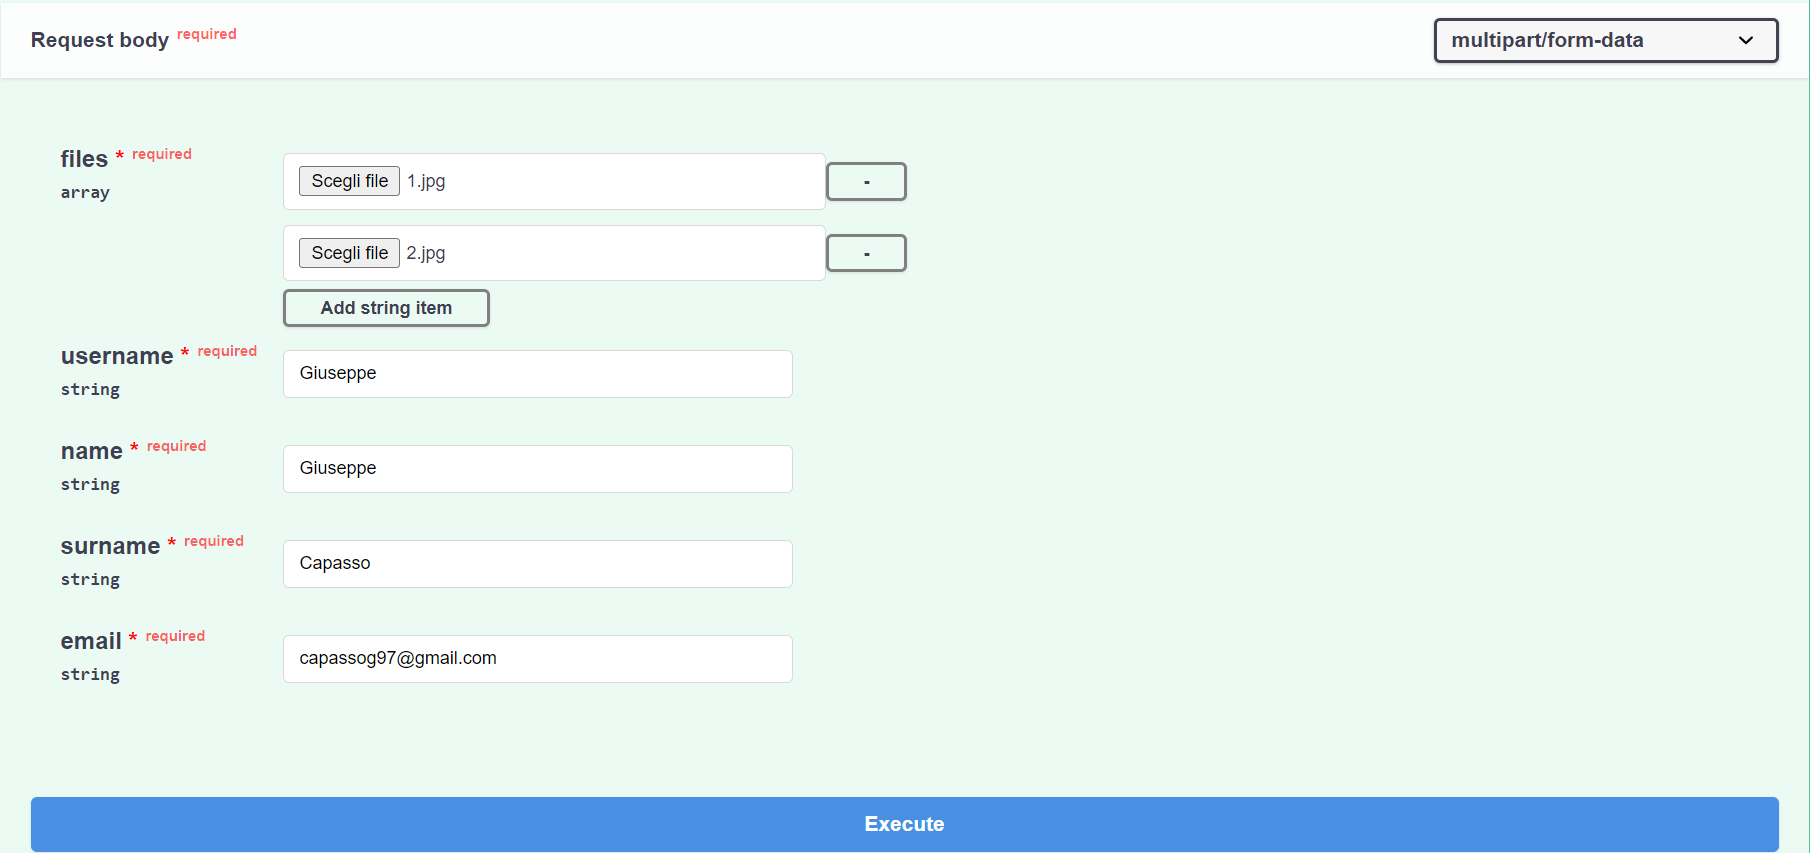
\includegraphics[width=\textwidth]{images/creazione_utente.png}
    \caption{Creazione utente}
    \label{fig:creazione_utente}
\end{figure}

\subsubsection{Login}
L'\textit{endpoint} login è utilizzato dai \textit{face scanner} per sbloccare o meno la serratura. I dispositivi inviano un'immagine JPEG che il server decodifica analogamente a quanto descritto in \cref{ss:creazione_utente} ed effettua un'operazione di \textit{matching} con gli \textit{encoding} precedentemente salvati con il modulo \textit{face\_recognition}. Nel caso di più match, viene applicata la funzione \textit{argmin} della libreria \textit{numpy} per scegliere il miglior risultato \textit{match} tra quelli ottenuti. Infine, con le coordinate ottenute (se esistono) sarà disegnato un rettangolo intorno ai volti riconosciuti nell'immagine di partenza e sarà ritornata al \textit{face scanner} per mostrare l'avvenuto riconoscimento all'utente (\cref{fig:tagged}). In ogni caso, l'immagine sarà salvata sul \textit{filesystem} in una cartella accessibile attraverso il web server. Infatti, per rendere visibili gli accessi basta navigare su un \textit{path} del tipo \textit{http://indirizzo\_server:porta/access/nome\_immagine.jpg}.
Infine, per alleggerire il carico sul database, gli \textit{encoding} vengono tenuti in \textit{Redis}.

\begin{figure}[ht]
    \centering
    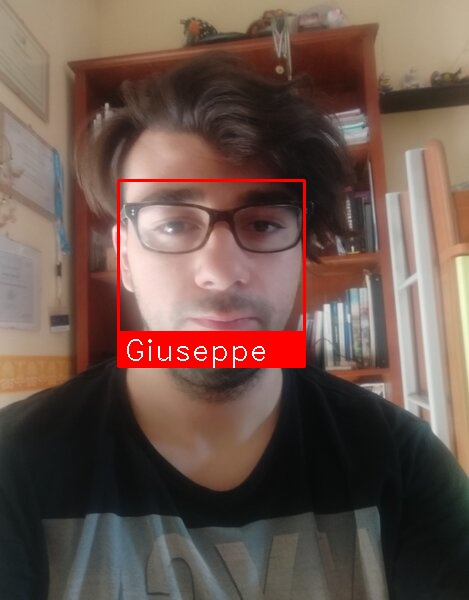
\includegraphics[scale=.4]{images/tagged.jpg}
    \caption{Immagine tornata dopo il login di un utente}
    \label{fig:tagged}
\end{figure}

\section*{Conclusioni}
\addcontentsline{toc}{section}{Conclusioni}
Il prototipo presentato in questo elaborato è fortemente dipendente dal protocollo HTTP che nasce per inviare informazioni di tipo testuale. Con i recenti sviluppi e la diffusione dei servizi REST, i \textit{web framework} sono diventati sempre più efficienti per le comunicazioni \textit{machine-to-machine}, ma si incontrano dei limiti quando bisogna trattare informazioni multimediali quali audio, immagini e video. Infatti, quando il server risponde con un'immagine ad una richiesta, HTTP non fornisce alcun modo di aggiungere \textit{metadata} all'immagine ritornata e, pertanto, risulta difficile controllare e/o modificare il comportamento dei \textit{face scanner} con informazioni aggiuntive (ad esempio mostrare messaggi particolari). \\
Dal punto di vista applicativo, il protocollo HTTP rende molto semplice lo sviluppo e il \textit{testing} di applicazioni che effettuano operazioni su database, ma poco efficiente dato l'\textit{overhead} aggiunto dalla struttura di richieste e risposte. D'altra parte, essendo molto utilizzato, il protocollo HTTP permette di integrare facilmente diverse modalità di autenticazione supportando diversi \textit{identity provider} (AD, OAuth2, etc.). Ciò permette di utilizzare \textit{database} di utenti già esistenti rendendo molto semplice l'integrazione con sistemi già esistenti.

Infine, il sistema presentato può offrire prestazioni degradate dopo un utilizzo di diversi anni. Infatti, salvando su un \textit{filesystem} classico le immagini degli accessi possono sorgere diversi problemi:
\begin{itemize}
    \item ottimizzazione dello spazio su disco: per questa problematica possono essere usati dei volumi fisici dedicati. Inoltre, conoscendo la dimensione media delle immagini, può essere configurata la dimensione dei blocchi dei dischi per ottimizzare l'uso dei settori;
    \item possibilità di \textit{query} lente: l'amministratore può desiderare di visionare gli accessi in un periodo temporale limitato. Se il \textit{database} contiene miliardi di record, la ricerca può diventare molto lenta. Con PostgreSQL, può essere applicato il \textit{table partitioning} che consente di dividere una tabella in più viste virtuali creando un indice sul campo data. Inoltre, queste viste virtuali possono essere distribuite su \textit{tablespace} diversi consentendo di utilizzare dischi più veloci per dati più recenti (acceduti più frequentemente);
    \item accoppiamento stretto tra registrazione dell'accesso e \textit{login}: nell'implementazione corrente, la procedura di \textit{login} fallisce se falliscono la scrittura del database dell'avvenuto accesso o il salvataggio dell'immagine. Per risolvere il problema, bisogna disaccoppiare i due eventi introducendo una coda asincrona (ad esempio un broker MQTT) delegando ad un servizio diverso la scrittura dei \textit{log} degli accessi. In questo modo, il processo di scrittura può essere più complicato e notificare altri servizi dell'avvenuto/tentativo di accesso e/o salvare in un servizio \textit{ad hoc} (in cloud o in locale) l'immagine;
\end{itemize}

\clearpage
\bibliographystyle{apacite}
\bibliography{refs}

\end{document}
